% !TeX spellcheck = en_US
\documentclass{article}

\usepackage{graphicx}

\usepackage[cp1250]{inputenc}
\usepackage[lastpage,user]{zref}
\usepackage[table,xcdraw]{xcolor}
\usepackage{pdfpages}
\usepackage{graphicx}
\usepackage[export]{adjustbox}
\usepackage{tabu}
\usepackage{enumerate}
\usepackage{color}


\begin{document}

\vspace*{3ex}
\begin{flushright}
{\large 28 March 2015}
\end{flushright}

\begin{flushleft}
{\large Lukasz W�jcik\\

}
\end{flushleft}

\hskip3cm

\begin{center}

\Large {\bf
	Individual project
}

\Large {\bf
	Cellular automaton
}

\Large {\bf 
	Technical project
}

\vskip2ex

\vspace{50pt}

\includegraphics[width=100mm]{images/mini.png} \\

\end{center}

\vskip20ex
\label{LastPage}
\begin{flushleft}
{\fontsize{10cm}{1em} {\bf Informations}\\
}
\end{flushleft}

\vskip2ex
\begin{flushleft}
{\huge Scheldue\\
}
\end{flushleft}
\begin{center}
\begin{table}[h]
\begin{tabular}{|l|l|}
\hline
\rowcolor[HTML]{BF6969} 
{\color[HTML]{000000} Date} & {\color[HTML]{000000} Stage} \\ \hline
2015-03-12                  & requirement specification    \\ \hline
2015-04-02                  & technical project            \\ \hline
2015-04-23                  & code of modules              \\ \hline
2015-04-30                  & version 0.98                 \\ \hline
2015-05-07                  & version 0.99                 \\ \hline
2015-05-14                  & version 1.0                  \\ \hline
2015-05-21                  & test report                  \\ \hline
2015-06-11                  & acceptation                  \\ \hline
\end{tabular}
\end{table}
\end{center}

\begin{flushleft}
{\huge Document metric\\
}
\end{flushleft}

\begin{table}[h]
\begin{tabular}{|
>{\columncolor[HTML]{BF6969}}l |l|l|l|l|l|}
\hline
\multicolumn{6}{|l|}{\cellcolor[HTML]{BF6969}\textbf{Document metric}}                                                                                                               \\ \hline
\textbf{Project:}       & \multicolumn{2}{l|}{Cellular automaton}          & \cellcolor[HTML]{BF6969}\textbf{Company:} & \multicolumn{2}{l|}{WUT}                                    \\ \hline
\textbf{Name:}          & \multicolumn{5}{l|}{Cellular Automata technical documentation}                                                                                           \\ \hline
\textbf{Topics:}        & \multicolumn{5}{l|}{Technical aspect of project}                                                                                                 \\ \hline
\textbf{Author:}        & \multicolumn{5}{l|}{Lukasz W�jcik}                                                                                                                         \\ \hline
\textbf{File:}          & \multicolumn{5}{l|}{cellular\_automata\_technical\_documentation}                                                                                        \\ \hline
\textbf{Version no:}    & 0.3 & \cellcolor[HTML]{BF6969}\textbf{Status:} & Designing                                 & \cellcolor[HTML]{BF6969}\textbf{Opening date:} & 2015-03-26 \\ \hline
\textbf{Summary:}       & \multicolumn{5}{l|}{Providing technical documentation.}\\ \hline
\textbf{Authorized by:} & \multicolumn{2}{l|}{Wladyslaw Homenda}           & \multicolumn{2}{l|}{\cellcolor[HTML]{BF6969}\textbf{Last modification date:}}              & 2015-04-08 \\ \hline
\end{tabular}
\end{table}
\begin{flushleft}
{\huge Changes\\
}
\end{flushleft}
\begin{table}[h]
\begin{tabular}{|l|l|l|l|}
\hline
\rowcolor[HTML]{BF6969} 
\multicolumn{4}{|l|}{\cellcolor[HTML]{BF6969}\textbf{History of changes}}     \\ \hline
\rowcolor[HTML]{E3DBDB} 
Version & Date       & Who           & Description                            \\ \hline
0.1     & 2015-03-26 & Lukasz W�jcik & Creation of technical documentation sections. Initial planning \\ \hline
0.2     & 2015-03-27 & Lukasz W�jcik & Creation of technical documentation.\\ \hline
0.21     & 2015-03-27 & Lukasz W�jcik & Correction of spelling mistakes. \\ \hline
0.3     & 2015-04-08 & Lukasz W�jcik & Correction of algorithm for adding rules.\\ \hline
\end{tabular}
\end{table}
\newpage
\tableofcontents
\vskip5ex
\begin{flushleft}
{\huge Short summary of documentation\\
}
\end{flushleft}
\Large\hspace{15pt}This document is a technical documentation of Cellular automation program.
\newpage

\section{Production model} \par
\Large\hspace{15pt}
Methodology used for implementation is a "Waterfall Model"
\begin{figure}[h!]
		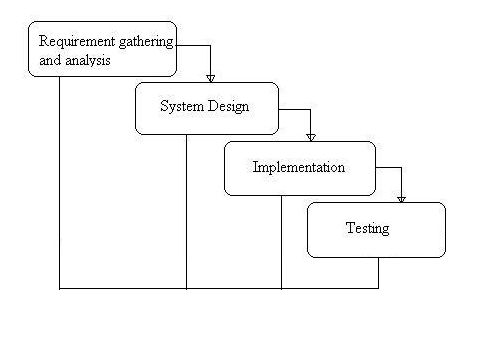
\includegraphics[width=1.0\textwidth, center]{images/waterfall_model.png}
		{Waterfall-model (In our case it end on testing)}
\end{figure}


This model is easy to understand and use. It is mostly used with relatively small project where all requirements are well understood (returning to earlier stages of project from e.g testing might be very expansive so it is better not to move to another stage without debugging). Each stage is completed one at a time so they are not overlapping.

\newpage
\section{Technologies} \par
\Large\hspace{15pt}
This application will be written in C\# language.Visual Studio 2013 will be used for an app development. WPF (Windows Presentation Foundation) will be used as a graphic engine. WPF is based on .NET 3. It gives nice tools to divide project on GUI and logical parts what helps in creating clean code. This application is destined for Windows Vista and higher. 



\section{Used data structures}
\Large\hspace{15pt}
To store grid data we will use two nested lists of cells object(or just boolean).In case of N x M grid, a list storing other lists will have length of N and inner lists will have length of M (each inner list represents one column of grid). In C\# exploring elements in List is as fast as in simple table but it gives way more tools. List is easy to expand/shrink and has many search functions already implemented.
\newpage
\section{Description of algorithms}
\Large\hspace{15pt} 
\begin{itemize}
	\item
		\hspace{15pt} {\Large \bf Algorithm for defining a new rule}
		\begin{enumerate}[I.]
		\item Open "Add/Edit rule" window.\\
		\item Click on "Add new" button to specify that a new rule will be added\\
		\textit{"All subrules which are manually added to a rule set are determining that cell is alive. All other possible rules are making cell dead by default."}
		\item Click on cells in a neighbors grid to choose those which will be included in counting active neighbors count, which will be refereed to as an "important" cell (It is also possible to select or deselect all rules by clicking on "Select all/Deselect all" button).\\
		\item Chose a number from 0 to N (number of cells in neighborhood included in process of determining a state of a particular cell) to define how many "imporatant" cells have to be alive to change state of a cell.\\
		\item Click on button indicating set of sub-rules to add to it a newly created sub-rule.\\
		\item Continue adding new sub-rules or click apply button to use newly created rule.
		
		\end{enumerate}
	 
	 \newpage
	  \item {\Large \bf  Algorithm for grid space wrapping}
	  
	  
	  
	 \textit{\large"Each cell in a matrix has its own index which represents its position in 2D space (coordinates [x,y]). In case where a cell from a neighborhood exceeds possible grid index we assume that top border and bottom border are connected and so are left and right border. After such assumptions we can imagine our matrix as a doughnut.All new values are saved to a copy of a grid."}
	 \\
	 	\begin{enumerate}[I.]
	 		\item If coordinate X of a neighborhood cell exceeds matrix from right side, calculate the difference between X coordinate and grid width and set a X coordinate to the value of a difference.
	 		\item If coordinate X of a neighborhood cell exceeds matrix from left side, set a value of an X coordinate to a sum of its starting value and grid width.
	 		\item If coordinate Y of a neighborhood cell exceeds matrix from bottom side, calculate the difference between Y coordinate and grid height and set Y coordinate to the value of a difference.
	 		\item If coordinate Y of a neighborhood cell exceeds matrix from the upper side, set a value of an y coordinate to a sum of its starting value and grid height.\\
	 		
	 		
	 		\textit{"Neighborhood cell may exceed both X and Y axis of the grid. In this situation both coordinates should be recalculated."}
	 		\\
	 	\end{enumerate}
	 \item  
	 	\hspace{15pt} {\Large \bf Algorithm for determining state of a cell by a rule.}
	 	\begin{enumerate}[I.]
	 	\item Do following procedures until sub-rule for living cell will be found or until the and of sub-rule list:
	 		\begin{enumerate}[a)]
	 		\item Iterate trough all cells in neighborhood and count a number of "important", living ones ("important" cells are defined by sub-rule).
	 		\item Check if obtained number is equal to the one expected by sub-rule.
	 		\item If obtained number is equal to needed value than return information that sub-rule for living cell can be applied and stop checking other sub-rules.
	 		\item If obtained number is not equal to needed value than check next sub-rule.
	 		\end{enumerate}
	 	\item If previous procedure returned information that there is a sub-rule which can be applied to a cell than change its state to living, otherwise change it to dead.	
	 	\end{enumerate}
	 	\newpage
	\item 
		\hspace{15pt} {\Large \bf Algorithm for creating new generation.}\\
		
		
		\textit{"For this procedure two matrices will be needed. One storing state values from current generation and second for a new generation. After computation of each generation they are switching places"}
		
		\begin{enumerate}[I.]
			\item For each cell in a current generation matrix do following procedures:
			\begin{enumerate}[a)]
				\item Calculate a new state of cell following algorithm determining a state of a cell.\\
				\item save a new state to a matrix storing states for a new generation		
			\end{enumerate}
			\item Set new generation matrix to a current generation matrix and redraw visualization of a grid.
		\end{enumerate}
		
		
\end{itemize}
\newpage
\section{Functionality}
{\large
	\begin{itemize}
	
	\item	
	Display visualization of cell movements - every step of components behavior must be
	shown on a grid.\\
	\item Change environment - by selecting them; there must be at least 3 types of
	environments: 4, 8, 24 points neighborhood. \\
	\item Introduce new rules - by adding new rules determining new behavior of cells. \\
	\item Change rules - by dynamically changing existing rules. \\
	\item Create new rules - by selecting neighborhood cells and how many of them should be
	alive in order to make the target cell either alive or dead.\\
	\item Select number of steps .\\
	\item Control simulation - by choosing options play, pause, stop or reset simulation. \\
	\item Observe movements step by step - by rewinding cells movement on click, depending on
	the selected number of steps. \\
	\item Change grid's size - by option to zoom in/zoom out the visualisation.\\
	\item Load known automaton - for example Langton's ant. \\	
	\item Display information - by showing for example time of simulation (in seconds), number
	of cells alive. \\			
	\end{itemize}
	}
\newpage
\section{Class diagram / program structure}
\Large\hspace{15pt} 
This class diagram is a simple visualization  of classes in our program. Person implementing these classes is free to divide them to smaller ones.
\begin{figure}[h!]
		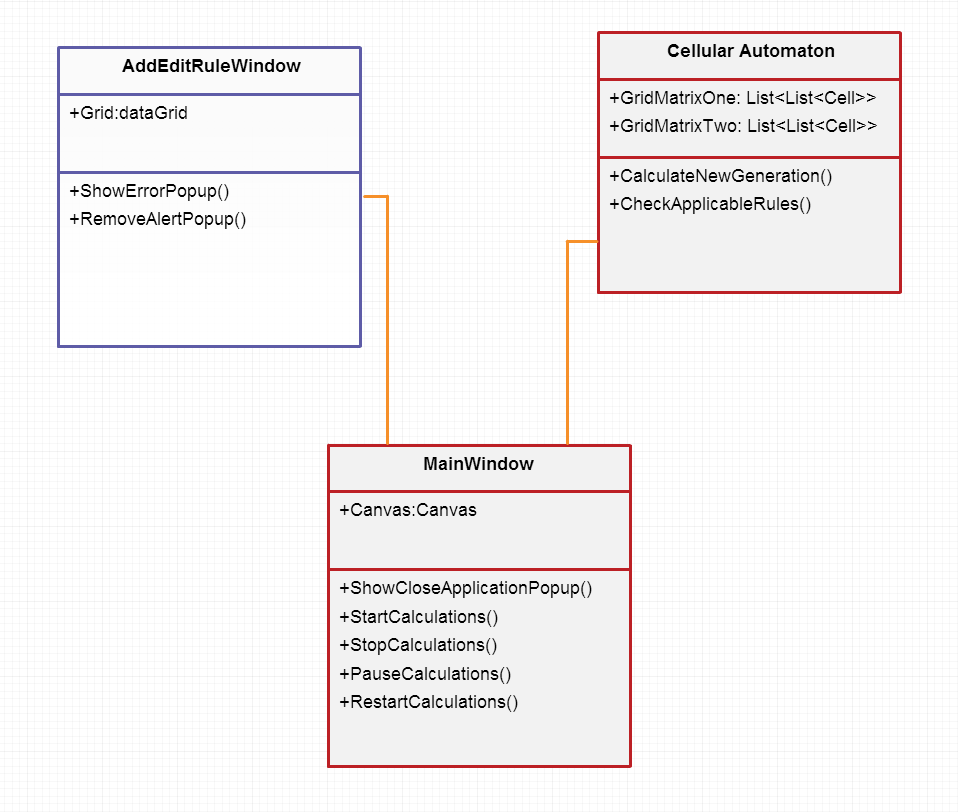
\includegraphics[width=1.5\textwidth, center]{images/Class_Diagram}
\end{figure}
\newpage
\section{Use cases}
Use case for user in main menu.
\begin{figure}[h!]
		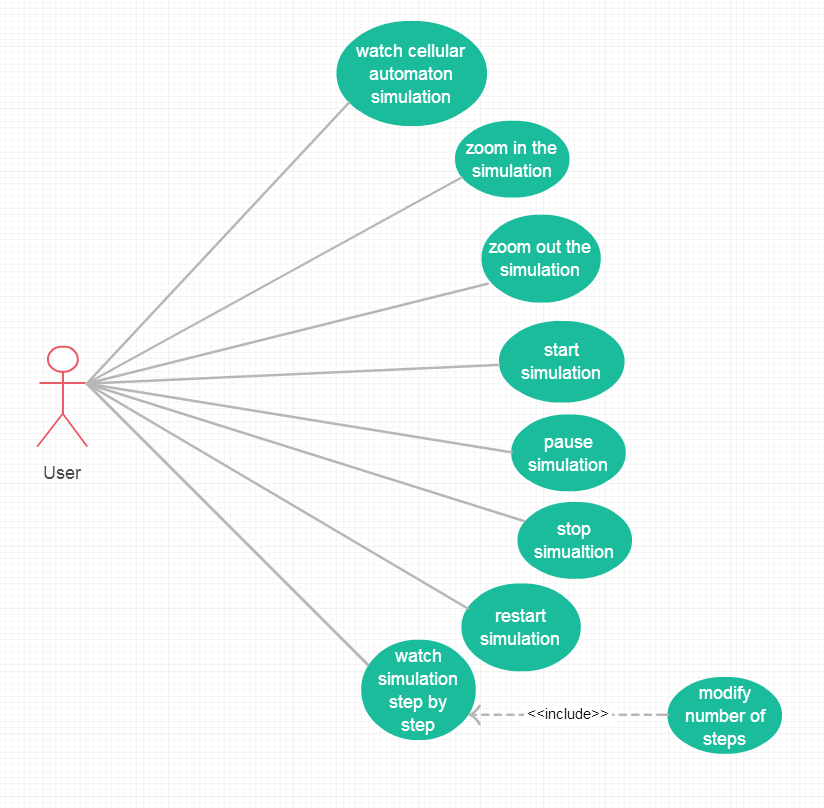
\includegraphics[width=1.3\textwidth, center]{images/user_usecase_diagram.png}
\end{figure}
\newpage
Use case for user in Add/Edit menu.
\begin{figure}[h!]
		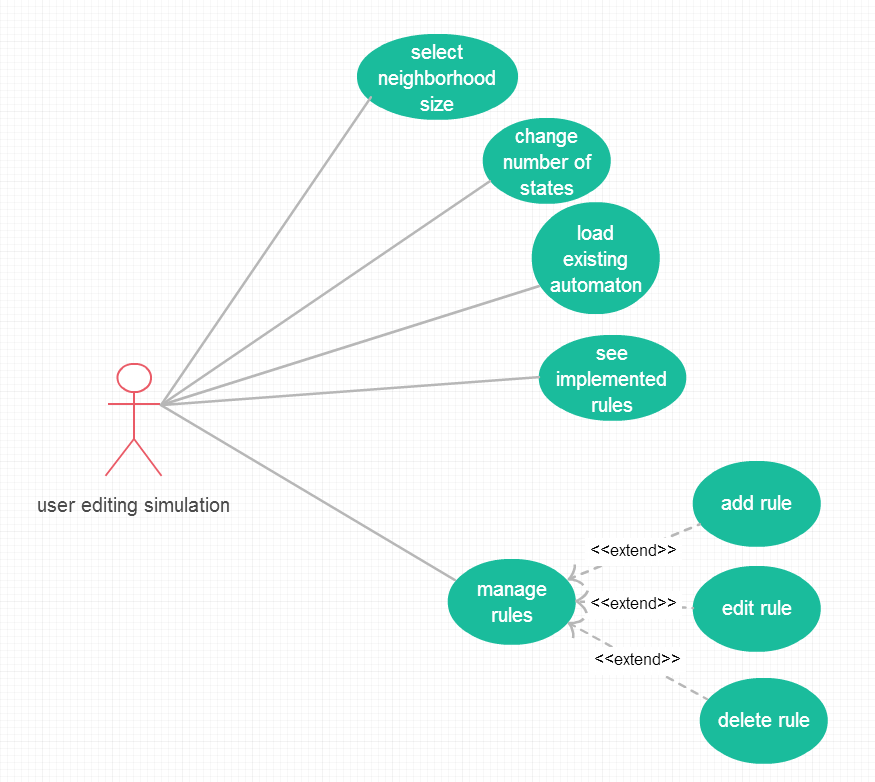
\includegraphics[width=1.3\textwidth, center]{images/user_editing_simulation_usecase_diagram.png}
\end{figure}


\newpage


\section{States diagram}
Simple state diagram describing behavior of program in general.
\begin{figure}[h!]
		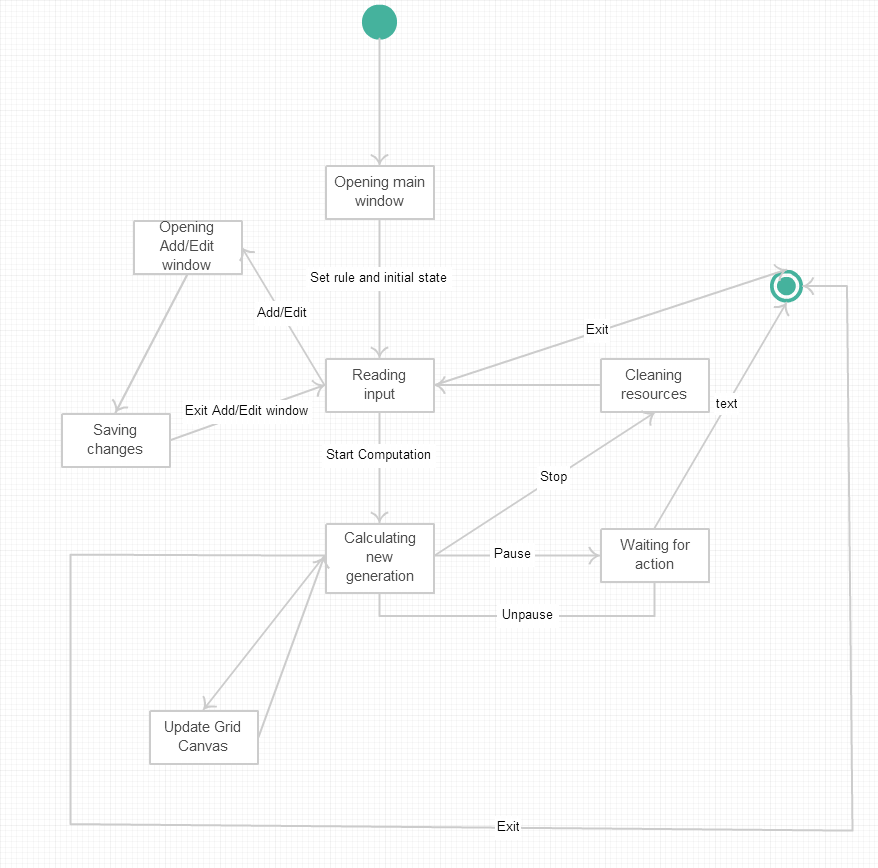
\includegraphics[width=1.3\textwidth, center]{images/state_diagram.png}
\end{figure}
\newpage

\section{Graphical user interface mock-up}
\textit{\large"Graphical user interface has been slightly modified since there won't be any possibility to manually determine rules for death of cell, hence there won't be any contradiction in applying rules."}
\begin{figure}[h!]
		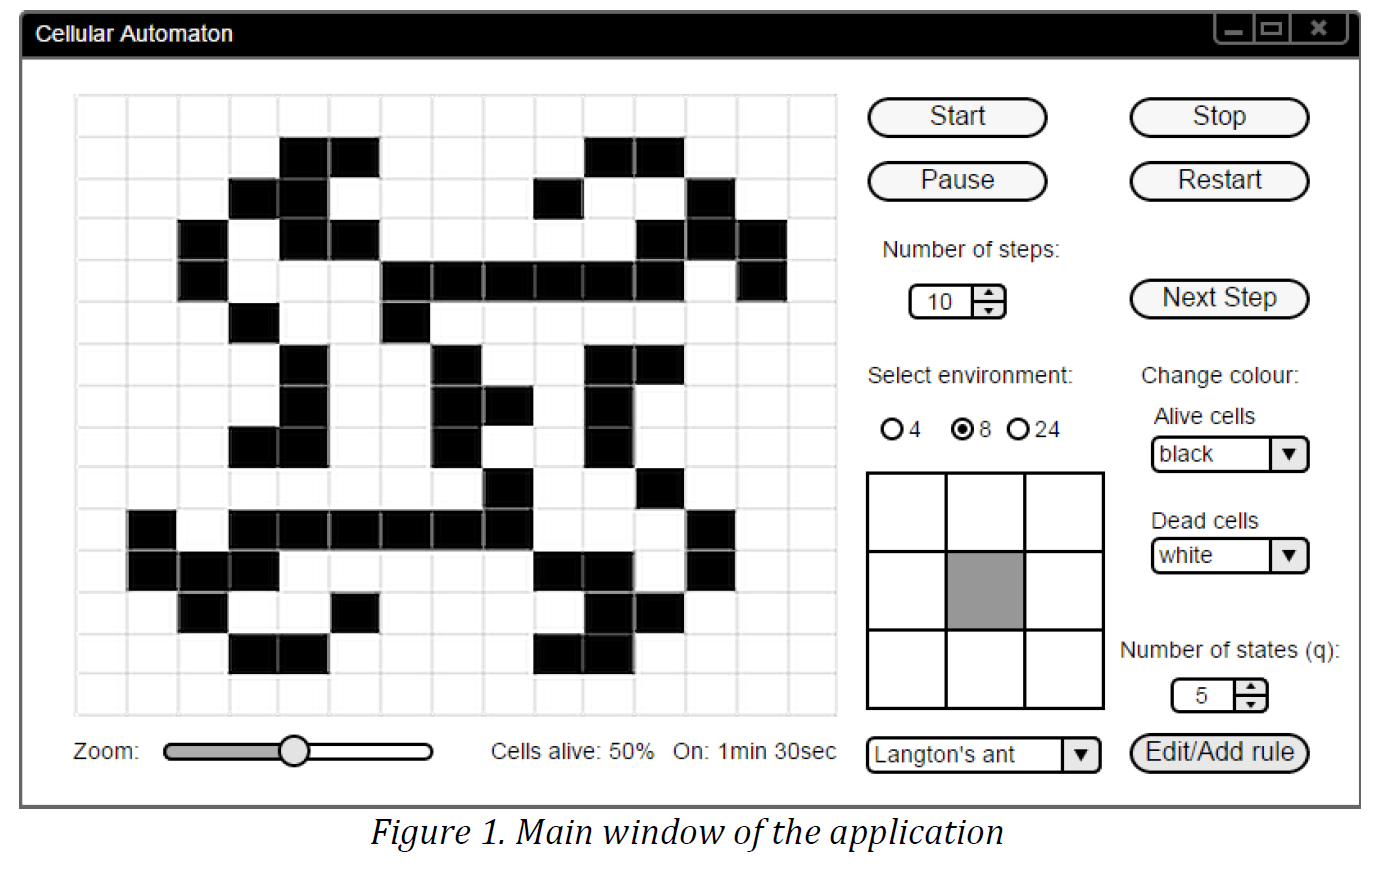
\includegraphics[width=1.0\textwidth, center]{images/Figure1.png}
\end{figure}
\begin{figure}[h!]
		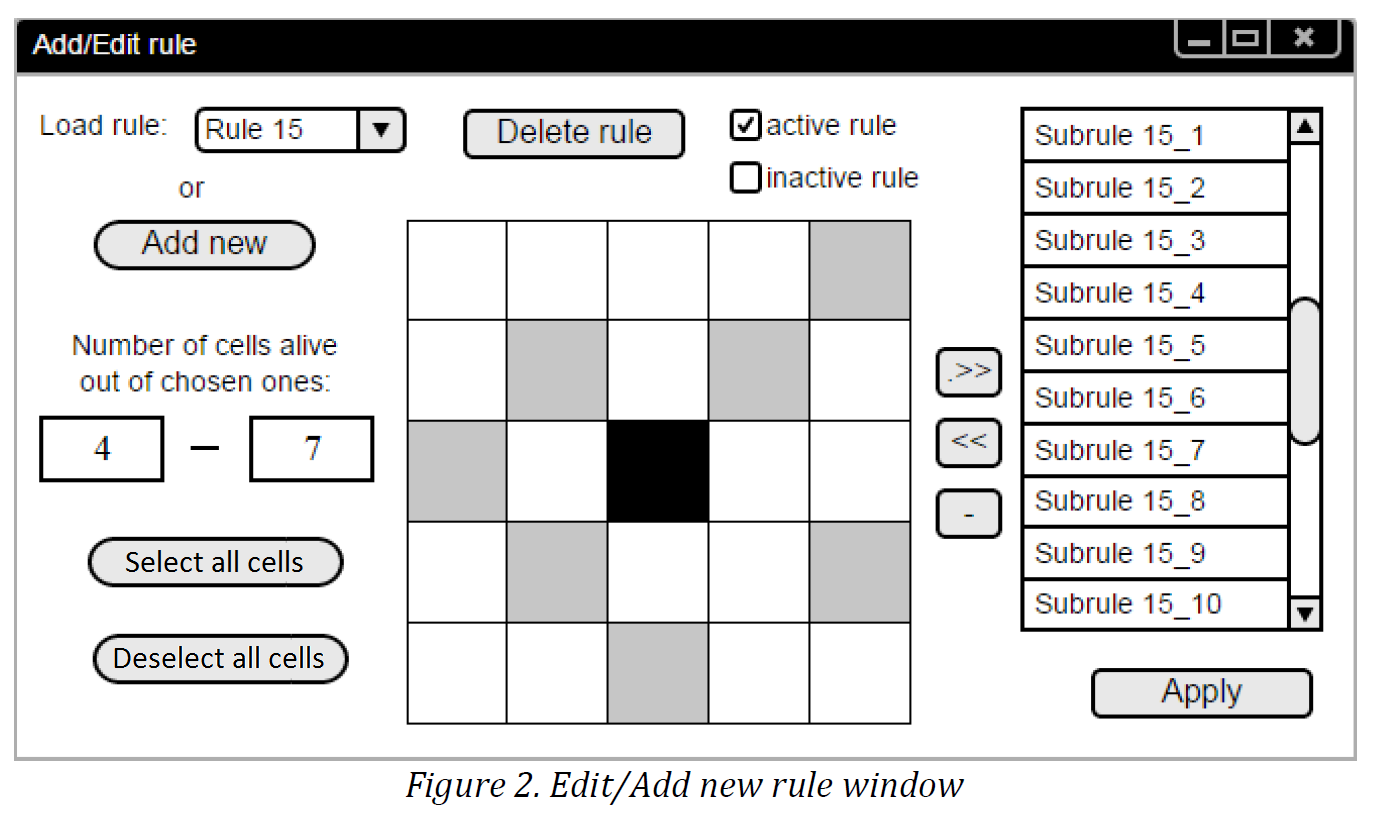
\includegraphics[width=1.0\textwidth, center]{images/Figure2.png}
\end{figure}
\iffalse
\begin{figure}[h!]
		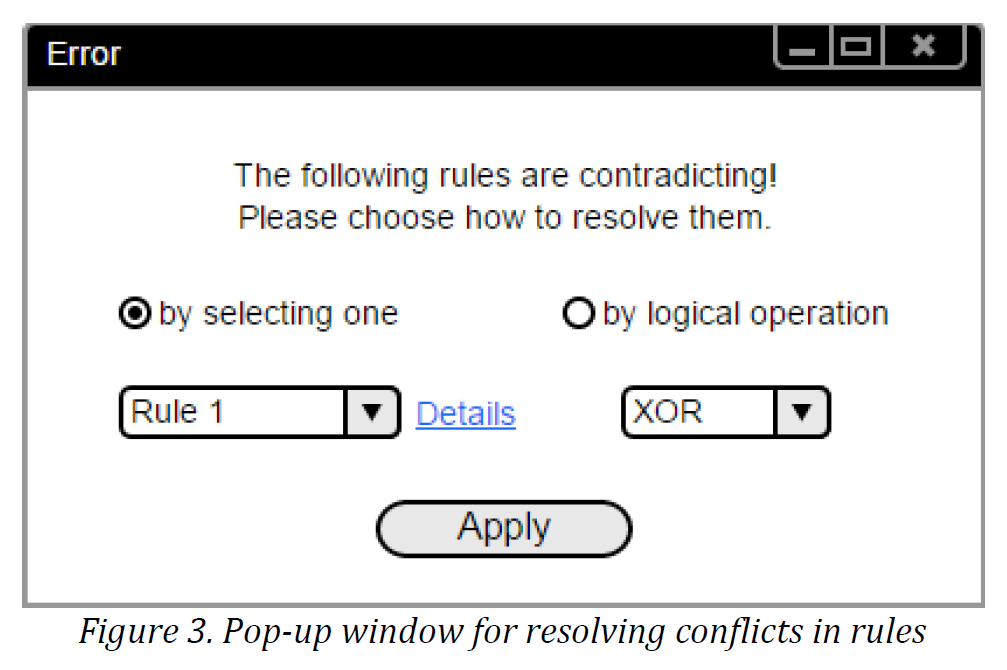
\includegraphics[width=0.8\textwidth, center]{images/Figure3.png}
\end{figure}
\begin{figure}[h!]
		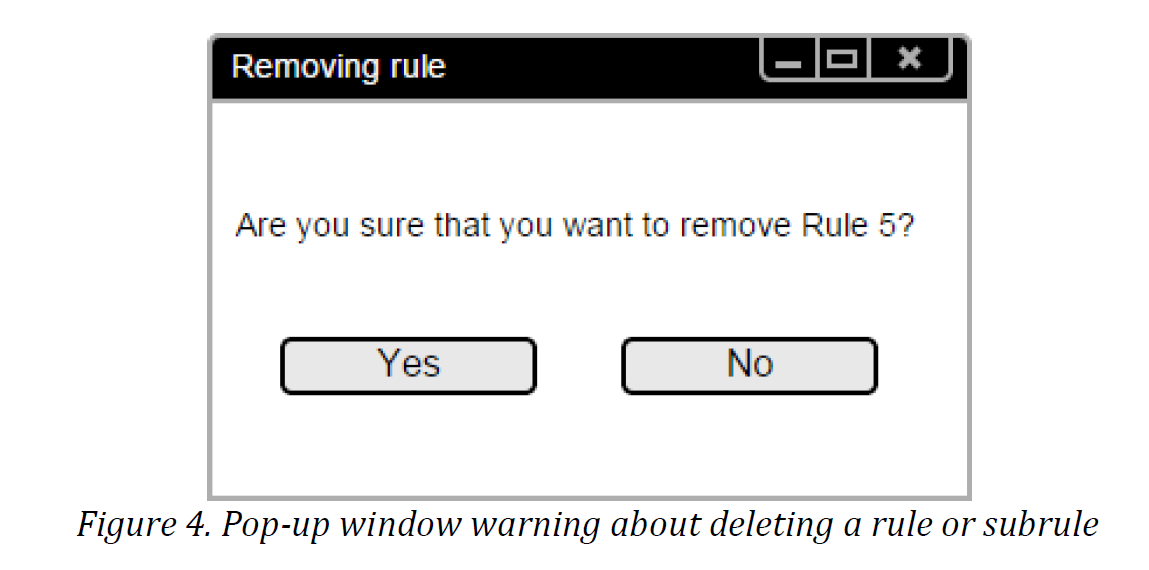
\includegraphics[width=1.0\textwidth, center]{images/Figure4.png}
\end{figure}

\begin{figure}[h!]
		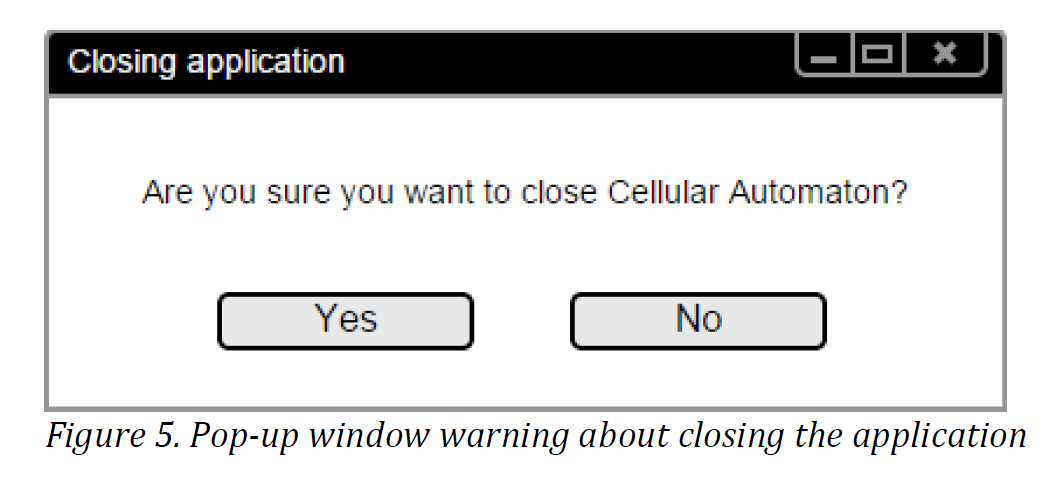
\includegraphics[width=0.8\textwidth, center]{images/Figure5.png}
\end{figure}
\fi
\newpage

\section {Summary}

This technical documentation is based on Business analysis made by Mai Viet Ba. I have made small changes in terms of functionality. User won't be able to manually create rules for death of a cell. User will be able to create rules which will change status of a cell to living and the rest of rules from rule set will cause death of a cell. Such changes will prevent any contradiction and will save a lot of computational power since it won't be needed to check all rules in a rule set. "Functionality" and "Graphical from business documentation has been modified and included in this document. 

Application created basing on this documentation should be very fast, user friendly and eye pleasing. The biggest drawback will be support for only one computer system (it also might be open through "Wine" on Linux but it's not an official solution so it might not work properly).


\end{document}
